\subsection{Temporal cycle consistency}
\begin{frame}[allowframebreaks]{Temporal cycle consistency}
    \textbf{Temporal Cycle Consistency} is a self-supervised learning approach that leverages the temporal structure of videos to learn representations by ensuring that transformations applied to video frames can be reversed.

    \begin{itemize}
        \item \textbf{Cycle Consistency:} The model learns to predict the optical flow between pairs of video frames, ensuring that the transformation can be reversed.
        \item \textbf{Applications:} Useful for tasks like tracking and correspondence learning.
        \item \textbf{Goal:} To learn robust representations that capture the temporal dynamics of video data.
    \end{itemize}
\framebreak
    \begin{figure}
        \centering
        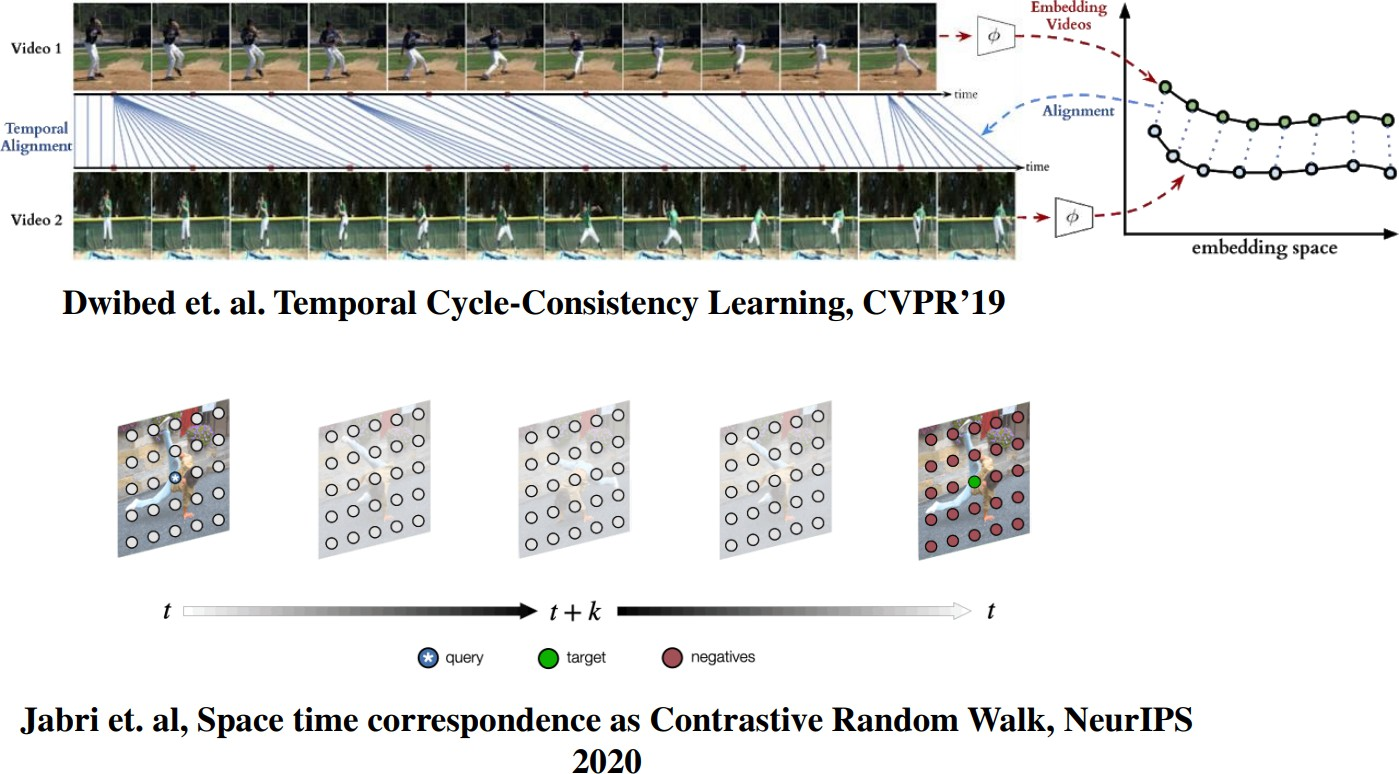
\includegraphics[width=1\textwidth,height=0.9\textheight,keepaspectratio]{images/video/slide_48_1_img.jpg}
    \end{figure}
\end{frame}